\chapter{Importação}

O InVesalius importa arquivos no formato DICOM, incluindo arquivos compactados (JPEG sem perdas e
com perdas) e arquivos no formato Analyze (Mayo Clinic)$^\copyright$.

\section{DICOM}

No menu \textbf{Arquivo}, clique na opção \textbf{Importar DICOM...}. Se preferir, use o atalho
do teclado \textbf{Ctrl + I}. A importação também pode ser acionada pelo ícone da barra de ferramentas
descrito na figura \ref{fig:import}.

\begin{figure}[!htb]
\centering

\includegraphics[scale=0.2]{file_import_original.png}
\caption{Atalho para Importar DICOM}
\label{fig:import}
\end{figure}

\hspace{.2cm}

Em seguida, selecione o diretório que contenha os arquivos DICOM, como na figura \ref{fig:win_folder}.
O InVesalius irá procurar por arquivos também em subdiretórios do diretório escolhido, caso existam.

\newpage

Clique em \textbf{OK}.

\begin{figure}[!htb]
\centering
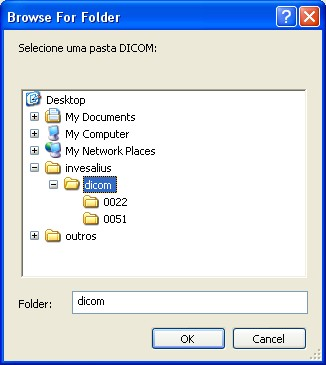
\includegraphics[scale=0.6]{ScreenHunter_04Dec311139.jpg}
\caption{Seleção de diretório}
\label{fig:win_folder}
\end{figure}

\hspace{.2cm}

Enquanto o InVesalius procura por arquivos DICOM no diretório, é exibido o progresso
do carregamento dos arquivos verificados, como ilustra a figura \ref{fig:ver_file}.

\begin{figure}[!htb]
\centering
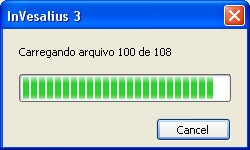
\includegraphics[scale=0.6]{ScreenHunter_03Dec311131.jpg}
\caption{Status de verificação e carregamento de arquivos}
\label{fig:ver_file}
\end{figure}

\newpage

Se arquivos DICOM forem encontrados, é aberta uma janela (figura \ref{fig:win_import})
para selecionar o paciente e a respectiva série que se deseja abrir. Também é possível
pular imagens para reconstrução.

\begin{figure}[!htb]
\centering
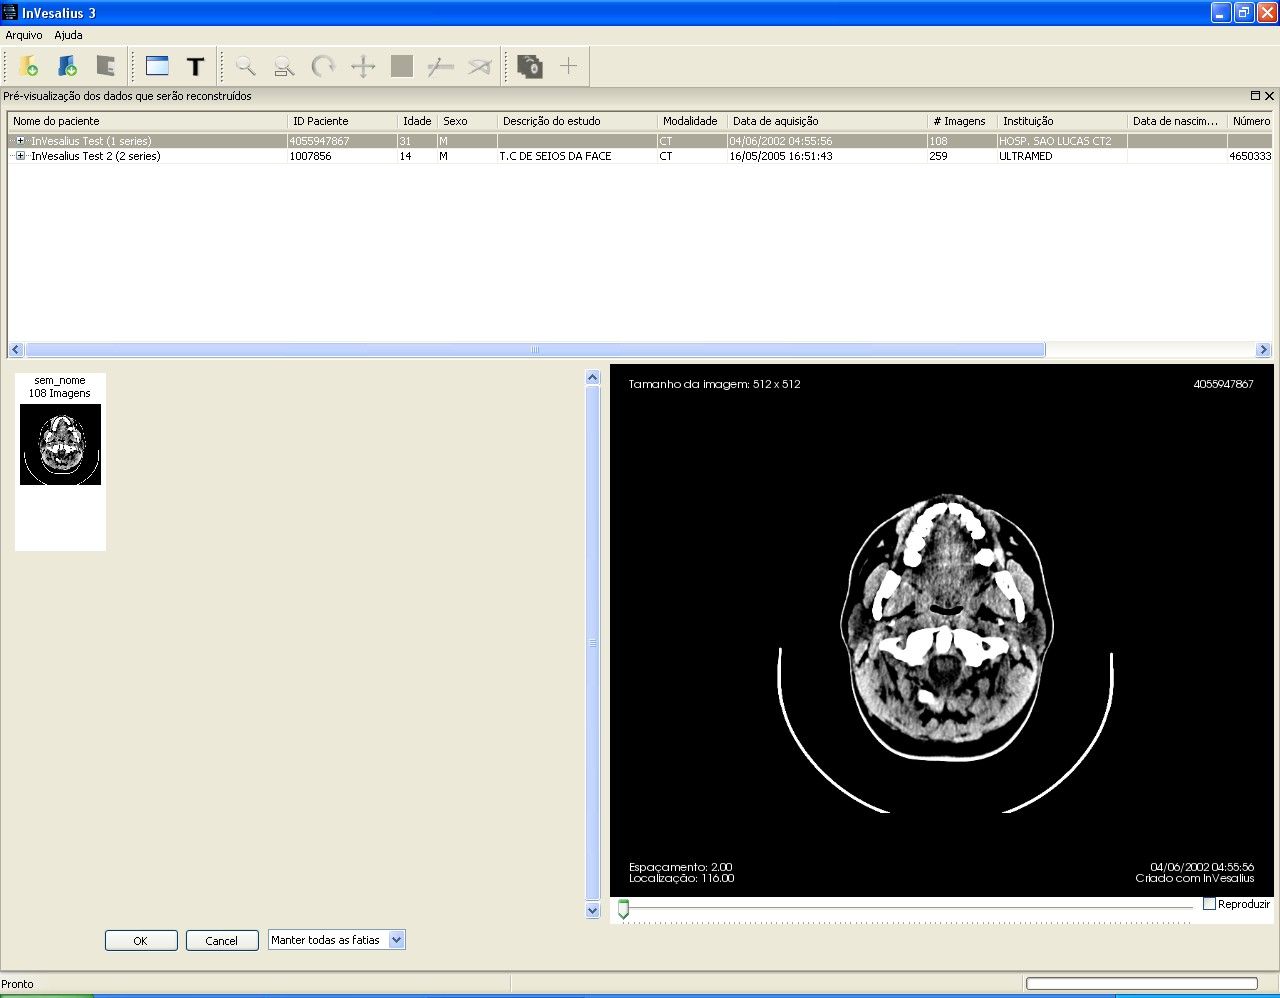
\includegraphics[scale=0.3]{ScreenHunter_06Dec311139.jpg}
\caption{Tela de importação}
\label{fig:win_import}
\end{figure}

\newpage

Caso deseje importar uma série com todas as imagens presentes, clique em "\textbf{+}" ao
lado do nome do paciente para expandir as séries a ele pertencentes. Dê um \textbf{clique duplo}
com o botão \textbf{esquerdo} do mouse sobre a descrição da série. Veja a figura
\ref{fig:import_serie}.

\begin{figure}[!htb]
\centering
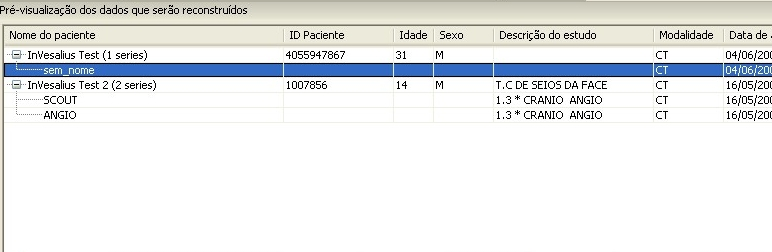
\includegraphics[scale=0.5]{ScreenHunter_08Dec311139_.jpg}
\caption{Seleção de série}
\label{fig:import_serie}
\end{figure}
 
%\hspace{.2cm}

Em alguns casos, em particular quando não se dispõe de um computador com memória e/ou
processamento satisfatórios para trabalhar com muitas imagens em uma série, pode ser
recomendável pular (ignorar) algumas delas. Para isso, clique \textbf{uma vez} com o botão
\textbf{esquerdo} do mouse sobre a descrição da série (figura \ref{fig:import_serie}) e selecione
quantas imagens serão puladas (figura \ref{fig:skip_image}). Clique em \textbf{OK}.

\begin{figure}[!htb]
\centering
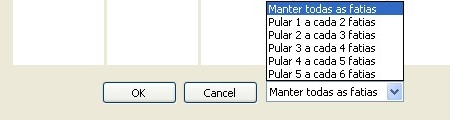
\includegraphics[scale=0.6]{ScreenHunter_13Dec311140_.jpg}
\caption{Pular imagens}
\label{fig:skip_image}
\end{figure}

%\hspace{.2cm}

Em ambos os procedimentos, será apresentada uma janela (figura \ref{fig:prog_recons}) com o progresso
da reconstrução (quando as imagens são empilhadas e interpoladas).

\begin{figure}[!htb]
\centering
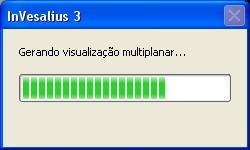
\includegraphics[scale=0.5]{ScreenHunter_14Dec311140.jpg}
\caption{Progresso da reconstrução}
\label{fig:prog_recons}
\end{figure}

\newpage

\section{Analyze}
Para importar arquivos no formato Analyze, basta ...